Higgs 有效势把一圈量子修正组织为常数背景场的 1PI 有效作用量。它适合研究真空位置和大场行为，但属于离壳对象，因此必须同时区分重整化尺度依赖、规范固定依赖和真正的物理极点量。

取中性径向背景
\begin{equation*}
\Phi_{\rm bg}
=\frac1{\sqrt2}\begin{pmatrix}0\\\varphi\end{pmatrix},
\qquad
\varphi_E\equiv\sqrt{\hbar c}\,\varphi,
\qquad [\varphi_E]=\mathrm J,
\end{equation*}
并定义 $\mu_E^2=(\hbar c)^2\mu_H^2$。树级势能密度为
\begin{equation*}
V_0(\varphi_E)
=\frac1{(\hbar c)^3}
\left[-\frac{\mu_E^2\varphi_E^2}{2}
+\frac{\lambda_H\varphi_E^4}{4}\right],
\end{equation*}
其量纲为 $\mathrm{J\,m^{-3}}$。

令背景依赖的静质量能量平方为
\begin{equation*}
\mathcal M_i^2(\varphi_E)\equiv[m_i(\varphi_E)c^2]^2,
\end{equation*}
并把重整化动量尺度 $\mu_{\rm DR}$ 对应到能量尺度
\begin{equation*}
E_{\rm R}\equiv c\mu_{\rm DR}.
\end{equation*}
在 Landau 规范中，保留第三代顶夸克 Yukawa 耦合作为主要费米子贡献时，所需背景质量为
\begin{align*}
\mathcal M_W^2&=\frac{g^2}{4}\varphi_E^2,&n_W&=6,\\
\mathcal M_Z^2&=\frac{g^2+g'^2}{4}\varphi_E^2,&n_Z&=3,\\
\mathcal M_t^2&=\frac{y_t^2}{2}\varphi_E^2,&n_t&=-12,\\
\mathcal M_h^2&=-\mu_E^2+3\lambda_H\varphi_E^2,&n_h&=1,\\
\mathcal M_G^2&=-\mu_E^2+\lambda_H\varphi_E^2,&n_G&=3.
\end{align*}
$n_i$ 已包含自旋、荷态、颜色多重度以及费米子行列式的负号。对常数背景做一圈展开时，真正的计算起点是各涨落场二次算符的高斯行列式。把费米子的负号以及自旋、荷态和颜色多重度统一收入 $n_i$，可以把所有粒子种类写成同一个母式
\begin{equation}
\boxed{
V_1(\varphi_E)
=\frac{\hbar c}{2}\sum_i n_i
\left(\frac{\mu_{\rm DR}}{\hbar}\right)^{2\epsilon}
\int\frac{\dd^d k}{(2\pi)^d}
\ln\!\left[k^2+\frac{\mathcal M_i^2(\varphi_E)}{(\hbar c)^2}\right],
\qquad d=4-2\epsilon .}
\label{eq:sm-one-loop-determinant-master-dp68}
\end{equation}
$n_i$ 对费米子取负值，因此\eqnrefs{eq:sm-one-loop-determinant-master-dp68} 已经包含玻色/费米的相对负号。对每个背景质量积分执行维数正则化并作 $\overline{\rm MS}$ 减除后，得到 Coleman--Weinberg 形式：
\begin{equation}
\boxed{
V_{\rm eff}(\varphi_E;E_{\rm R})
=V_0(\varphi_E)
+\frac1{64\pi^2(\hbar c)^3}
\sum_i n_i\mathcal M_i^4(\varphi_E)
\left[\ln\frac{\mathcal M_i^2(\varphi_E)}{E_{\rm R}^2}-c_i\right]
+\mathcal O(\hbar^2).}
\label{eq:sm-coleman-weinberg-si-dp12}
\end{equation}
其中标量的 $c_i=3/2$，质量矢量场的横向规范不变贡献在常用协变规范中对应 $c_i=5/6$。当某个背景曲率本征值变成负值时，对数产生虚部；它表示该均匀背景对相应涨落不稳定，而不是一个可直接解释为静态能量密度的复数“势能”。

\eqnrefs{eq:sm-coleman-weinberg-si-dp12} 是前章 1PI Callan--Symanzik 方程在常数 Higgs 背景上的特化：
\begin{equation}
\boxed{
\left[
E_{\rm R}\frac{\partial}{\partial E_{\rm R}}
+\sum_a\beta_{g_a}\frac{\partial}{\partial g_a}
-\gamma_\Phi\varphi_E\frac{\partial}{\partial\varphi_E}
\right]V_{\rm eff}=0.}
\label{eq:sm-effective-potential-rg-equation-dp12}
\end{equation}
当 $\varphi_E\gg v_E$ 时，固定阶中的 $\ln(\varphi_E^2/E_{\rm R}^2)$ 可能很大。选取 $E_{\rm R}=\kappa\varphi_E$、$\kappa=\mathcal O(1)$ 可以把大对数转移到运行耦合中；忽略质量项后，主导的重整化群改进形式为
\begin{equation*}
V_{\rm eff}(\varphi_E)
\simeq\frac{\lambda_H(E_{\rm R})}{4(\hbar c)^3}
Z_\Phi^4(E_{\rm R})\varphi_E^4,
\qquad
Z_\Phi(E_{\rm R})
=\exp\!\left[-\int^{E_{\rm R}}\gamma_\Phi(E)\dd\ln E\right].
\end{equation*}
因此大场稳定性取决于运行的 $\lambda_H$、匹配修正和场反常维数，而不是树级势中某个固定的 $\lambda_H$ 数值。

有效势的第二个关键限制来自规范依赖。规范固定参数 $\xi$ 改变时，离壳有效势的曲线形状一般会改变；但这种改变不能让同一个物理真空得到不同的可观测预测。BRST 对称性把两种变化联系起来：一方面显式改变 $\xi$，另一方面同时沿背景场坐标 $\varphi_E$ 作一个由函数 $C(\varphi_E,\xi)$ 决定的补偿移动。二者在有效势上的总变化必须相消，因此常数背景满足
\begin{equation}
\boxed{
\frac{\partial V_{\rm eff}(\varphi_E,\xi)}{\partial\xi}
+C(\varphi_E,\xi)
\frac{\partial V_{\rm eff}(\varphi_E,\xi)}{\partial\varphi_E}=0.}
\label{eq:sm-nielsen-identity-dp12}
\end{equation}
这个把规范参数变化与背景场重参数化联系起来的关系称为\emph{Nielsen 恒等式}。若 $\varphi_\star(\xi)$ 满足量子驻点条件 $\partial_{\varphi_E}V_{\rm eff}=0$，则链式法则与\eqnrefs{eq:sm-nielsen-identity-dp12} 给出
\begin{align*}
\frac{\dd}{\dd\xi}V_{\rm eff}(\varphi_\star(\xi),\xi)
&=\partial_\xi V_{\rm eff}
+\frac{\dd\varphi_\star}{\dd\xi}\partial_{\varphi_E}V_{\rm eff}\\
&=\left(-C+\frac{\dd\varphi_\star}{\dd\xi}\right)
\partial_{\varphi_E}V_{\rm eff}\\
&=0.
\end{align*}
因此驻点势值满足
\begin{equation}
\boxed{
\frac{\dd}{\dd\xi}
V_{\rm eff}(\varphi_\star(\xi),\xi)=0.}
\label{eq:sm-nielsen-stationary-value-dp68}
\end{equation}
驻点处的有效势值因而与 $\xi$ 无关；对驻点条件 $\partial_{\varphi_E}V_{\rm eff}(\varphi_\star,\xi)=0$ 取 $\xi$ 的全导数，再用 Nielsen 恒等式对 $\varphi_E$ 的导数，可在 $\partial_{\varphi_E}^2V_{\rm eff}\neq0$ 时一行得到
\begin{equation*}
\frac{\dd\varphi_\star}{\dd\xi}=C(\varphi_\star,\xi).
\end{equation*}
而具有规范依赖。因此任意规范下的 $\partial_{\varphi_E}^2V_{\rm eff}$ 不能直接认作物理 Higgs 极点质量；极点质量和衰变振幅必须由完整的在壳 1PI 方程定义。

\begin{figure}[htbp]
\centering
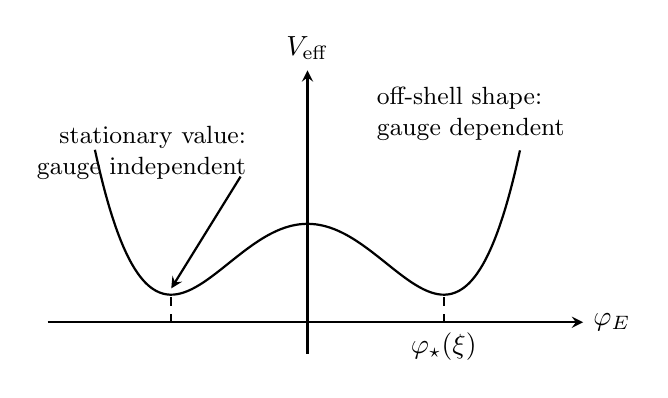
\begin{tikzpicture}[>=stealth,thick,line label/.style={fill=white,fill opacity=.96,text opacity=1,inner sep=1.15pt}]
\draw[->] (-3.3,0) -- (3.5,0) node[right]{$\varphi_E$};
\draw[->] (0,-.4) -- (0,3.2) node[above]{$V_{\rm eff}$};
\draw[smooth,domain=-2.7:2.7,samples=120] plot (\x,{0.10*(\x*\x-3)^2+0.35});
\draw[dashed] (-1.73,0)--(-1.73,.35);
\draw[dashed] (1.73,0)--(1.73,.35);
\node[below] at (1.73,0){$\varphi_\star(\xi)$};
\node[align=left,anchor=west,font=\small] at (0.75,2.65){off-shell shape:\\gauge dependent};
\node[align=right,anchor=east,font=\small] at (-0.65,2.15){stationary value:\\gauge independent};
\draw[->] (-0.85,1.85)--(-1.73,.43);
\end{tikzpicture}
\caption{有效势是离壳 1PI 对象，其曲线形状和驻点坐标一般依赖规范固定参数。Nielsen 恒等式保证量子驻点处的有效作用量值不随规范参数改变；物理质量仍需由完整极点条件定义。}
\label{fig:sm-nielsen-effective-potential-dp12}
\end{figure}

真空稳定性的微扰陈述必须同时带有尺度与规范控制。若在给定匹配方案和微扰阶数下，重整化群改进的有效四次耦合在某个能标区域变负，则大场方向可能低于电弱真空；但“$\lambda_{\rm eff}$ 的零点”本身不是严格的规范不变量。真正的可观测结论应通过真空隧穿作用量、寿命或其他规范一致的构造表达，并要求
\begin{equation*}
\epsilon_{\rm loop}
\sim\frac{\max(g_s^2,g^2,g'^2,y_t^2,\lambda_H)}{16\pi^2}\ll1,
\qquad
\left|\ln\frac{\varphi_E}{E_{\rm R}}\right|=\mathcal O(1),
\end{equation*}
否则必须加入更高圈重整化群改进或非微扰信息。
